% Options:
% withid: adds a header line for writing the student's ID (if a value is given, will limit the number of boxes)
% anonymous: replaces student name fieds by an anonimity number (if a value is given, it specifies the number of boxes)
%
% We recommend to keep the twoside option as it allows to add a specific header (student' name) on each new page.
%\documentclass[a4paper,twoside,anonymous]{correctexam}
\documentclass[a4paper,twoside,withid=8]{correctexam}

% packages already loaded: graphicx, geometry, listings, lastpage, fancyhdr, xcolor, mathpazo, ifthen, xstring, qcm, enumitem, etoolbox, cleveref

\usepackage[T1]{fontenc}
\usepackage[final,activate={true,nocompatibility},kerning=true,spacing=true]{microtype}
\usepackage[english,french]{babel}
\usepackage[scaled=0.9]{DejaVuSansMono}
\usepackage{lipsum} % For demo. To remove
\usepackage{tikz}

% You can adjust the line spread of the font used in this document (mathpazo).
%\linespread{1.05}

% You can override the default page dimensions, mainly left and right (touching the other parameters may break the template):
%\geometry{bottom=0.5cm, top=-1cm, left=1.3cm, right=1.3cm, headheight=5cm, includefoot, includehead}

% You can customise the centered footpage:
%\cfoot[\large\thepage~~/~~\pageref{LastPage}]{\large\thepage~~/~~\pageref{LastPage}}
% but do not change the \lhead, \rhead, \lfoot, \rfoot, and \chead as they are used for page detection and IDs

% CAUTION: this class sets the 'fboxsep' length to '0', which breaks spacing in the '\fbox' command.
% This affects packages that rely on '\fbox', such as the 'minted' package with the 'frame' option'
% A fix for 'minted' is to set 'framesep=5pt' to replace the missing spacing.


\title{\vspace*{-1cm}\huge Title}
\author{2022-2023\\[0.1cm]
Course handouts and lecture notes authorized\\[0.1cm]
Duration: 2 hours\\[0.1cm]
This exam has \pageref{LastPage} pages
}
\date{}


\begin{document}


% Creates the exam header
\maketitle

% The template contains several exam commands:
% \exerciceExam{number}{title} creates a section dedicated to a given exercice. Replace 'number' by the number of points of the exercise, 'title' is the title of the exercice (if no title, do not forget to put {})

% \questionExam{text} creates a numbered question. Replace 'text' by the title of the question.

% \begin{qcmExam}\end{qcmExam} creates a QCM environment

\begin{center}
\noindent\fbox{\parbox{\textwidth}{\centering\textbf{Write your answers directly inside the reply boxes, in this examen sheet. \\
Do not go beyond these areas. Do not forget to write your name on each sheet.}}}
\end{center}


\exerciceExam{5}{}

%\questionExam{\lipsum[1][1]}

\questionExam[q.label222]{First Question}

\cref{q.label222}

\exerciceExam{4}{}

\questionExam{\lipsum[1][1]}

% First argument: color (optional, by default black). The color of the dots. Put white for no dot.
% Second argument: the line spacing
% Third argument: the number of lines
% Fourth argument: the number of columns
\answerExam[gray]{1.5}{2}{1}

\questionExam{\lipsum[1][2]}

\questionExam[q.label2]{\lipsum[1][2]}

\answerExam[gray]{1.5}{4}{2}

\exerciceExam{4}{}


% A question can have a label:
\questionExam[q.mylabel]{\lipsum[1][3]}

% You can use the question's label like this:
\textbf{Reference to \cref{q.mylabel}}
% Warning: there is an issue when using question's label and section/sub-section.

\answerExam[white]{1.5}{8}{1}

\newpage

% \inlineAnswerBox as one argument: the length of the box (computed in number of characters). By default 10 characters.
% You can change the size of the answer box with text size commands: {\Large \inlineAnswerBox{}}
\questionExam{Complete the following text:}

You can also write some text with inline boxes \inlineAnswerBox{} that students must complete \inlineAnswerBox[5]{}.

\answerExam[white]{1.5}{8}{1}

% Be careful, if you use inlineAnswerBox inside a questionExam, you have to manually reinit the sub-question counter:
\questionExam{\setcounter{subquestioncounter}{1}You can also write some text with inline boxes \inlineAnswerBox{} that students must complete \inlineAnswerBox[5]{}.}


\exerciceExam{8}{}

\questionExam{Which color?}

\begin{qcmExam}
	\item blue
	\item red
\end{qcmExam}

\questionExam{Which form?}

\begin{qcmExam}
	\item rectangular
	\item triangular
\end{qcmExam}



\medskip


\questionExam{\lipsum[1-2]}

\answerExam[white]{1.5}{18}{1}

\newpage

\questionExam{\lipsum[3-4]}

\answerExam[white]{1.5}{18}{1}



% You can also create an answer box with a picture or some text, or code (lstlistings does not work here) to complete inside the box:
\answerExamContent{%
~\\
\hspace*{0.2cm}\texttt{void saisirEspece (}
\vspace*{1cm}

\hspace*{1cm}\texttt{printf("Saisir le nom et le prénom\textbackslash n");}
\vspace*{3cm}

\hspace*{1cm}\texttt{printf("Saisir une espèce\textbackslash n");}
\vspace*{4cm}
}


\answerExamContent{%
\tikz \draw (0,0) rectangle (3,4);
\begin{tikzpicture}%
	\draw (0,0) rectangle (3,5);
\end{tikzpicture}%
}


\answerExamContent{%
\begin{center}
	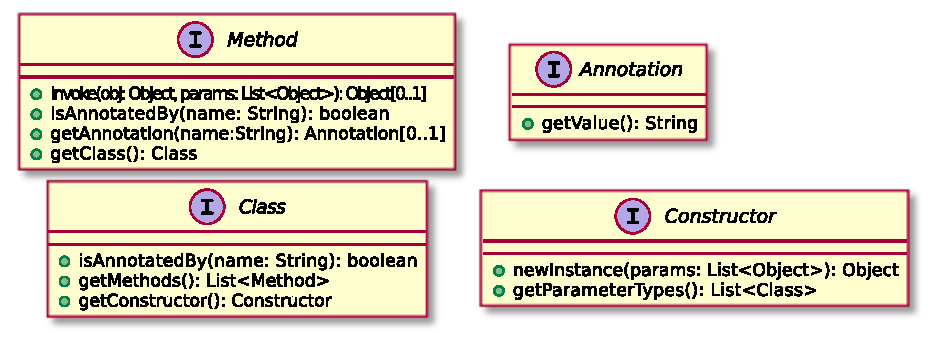
\includegraphics{diag.pdf}%
\end{center}
}


% Questions can also be created with a questionExamBlock environment.
% This ensures the question will be displayed on the same page as the environment content.
% For instance, this can be used to avoid starting a new page on an answer box.
\begin{questionExamBlock}{\lipsum[5]}
	\answerExam[white]{1.5}{18}{1}
\end{questionExamBlock}

% Similar to regular questions, a label can be set on a questionExamBlock.
\begin{questionExamBlock}[q.otherlabel]{\lipsum[6][1]}
	\answerExam[white]{1.5}{10}{1}
\end{questionExamBlock}

\textbf{Reference to \cref{q.otherlabel}}


\end{document}
